\documentclass[11pt]{article}
\usepackage[utf8]{inputenc}
\usepackage[T1]{fontenc}
\usepackage{minted}
\usepackage{graphicx}
\usepackage{hyperref}

\author{Student: Sean Wang, szw87 \\ Professor: Mohit Tiwari, Antonio Espinoza \\ Department of Electrical \& Computer Engineering \\ The University of Texas at Austin}
\date{\today}
\title{EE379K Enterprise Network Security Lab 2 Report}
\hypersetup{
 pdfauthor={Student: Sean Wang, szw87 \\ Professor: Mohit Tiwari, Antonio Espinoza \\ Department of Electrical \& Computer Engineering \\ The University of Texas at Austin},
 pdftitle={EE379K Enterprise Network Security Lab 2 Report},
 pdfkeywords={},
 pdfsubject={},
 pdfcreator={},
 pdflang={English}}

\begin{document}

\maketitle
\section*{Part 1 - Vulnerable Web-Apps}
\subsection*{1a - Containers}
\subsubsection*{PHP Injection}
The Damn Vulnerable Web App in Docker was setup on low difficulty by following the guide~\cite{dvwa}. Then, a
PHP file (\verb|part1/injection.php|) was uploaded to the web app, and could then be loaded and executed when navigated to. This PHP script
prints the path to the current directory, the contents of the current directory, the contents fo the root, and the number of processes
running in the system. The output of the script onto the webpage is shown below:
\begin{minted}{bash}
  Path to current directory:
  /var/www/html/hackable/uploads
  
  Contents of current directory:
  . .. dvwa_email.png injection.php
  
  Contents of root:
  . .. .dockerenv bin boot dev etc home lib lib64 main.sh
  media mnt opt proc root run sbin srv sys tmp usr var
  
  Number of processes running:
  17
\end{minted}
The server's view of the filesystem has a few differences from running \verb|ls /| from the VM's terminal. For example, it shows files
that are normally hidden, such as \verb|.|, \verb|..|, and \verb|.dockerenv|. The files and directories it doesn't show that
\verb|ls /| shows include \verb|cdrom/|, \verb|initrd.img|, \verb|initrd.img.old|, \verb|lib32/|, \verb|libx32/|, \verb|lost+found/|,
\verb|snap/|, \verb|swapfile|, \verb|vmlinuz|, \verb|vmlinuz.old|. Additionally, running \verb=ps aux --no-headers | wc -l= from the
VM's terminal resulted in 223 instead of 17. This difference is due to how Docker creates and manages containers. Docker utilizes the
Linux kernel's cgroups and namespaces in order to manage and monitor resource allocation, and utilizes the C library, \verb|runC|,
that gives each container its own root file system, similar to a \verb|chroot jail|~\cite{codementor,demystify}. As such, the root of
the filesystem seen by the Docker container and the VM are not the same filesystem, explaining the difference in output of \verb|ls /|.
Additionally, through the use of namespaces, Docker has isolated the processes inside the container from the processes of the VM
running Docker.
\subsubsection*{Content Security Policy Bypass}
On the Content Security Policy Bypass (CSP Bypass) page, there is a textbox that allows external scripts from certain allowed sites
to be run. In order to execute Javascript that creates a popup alert, a simple line of Javascript was inserted into a pastebin:
\begin{minted}{javascript}
  alert("this is a popup window");
\end{minted}
Then, by inserting the pastebin link to the raw text, \verb|https://pastebin.com/raw/wENwXfBR|, and pressing the include button, a popup
was generated, like in Figure~\ref{fig:CSP}.
\begin{figure}[!h]
  \centering
  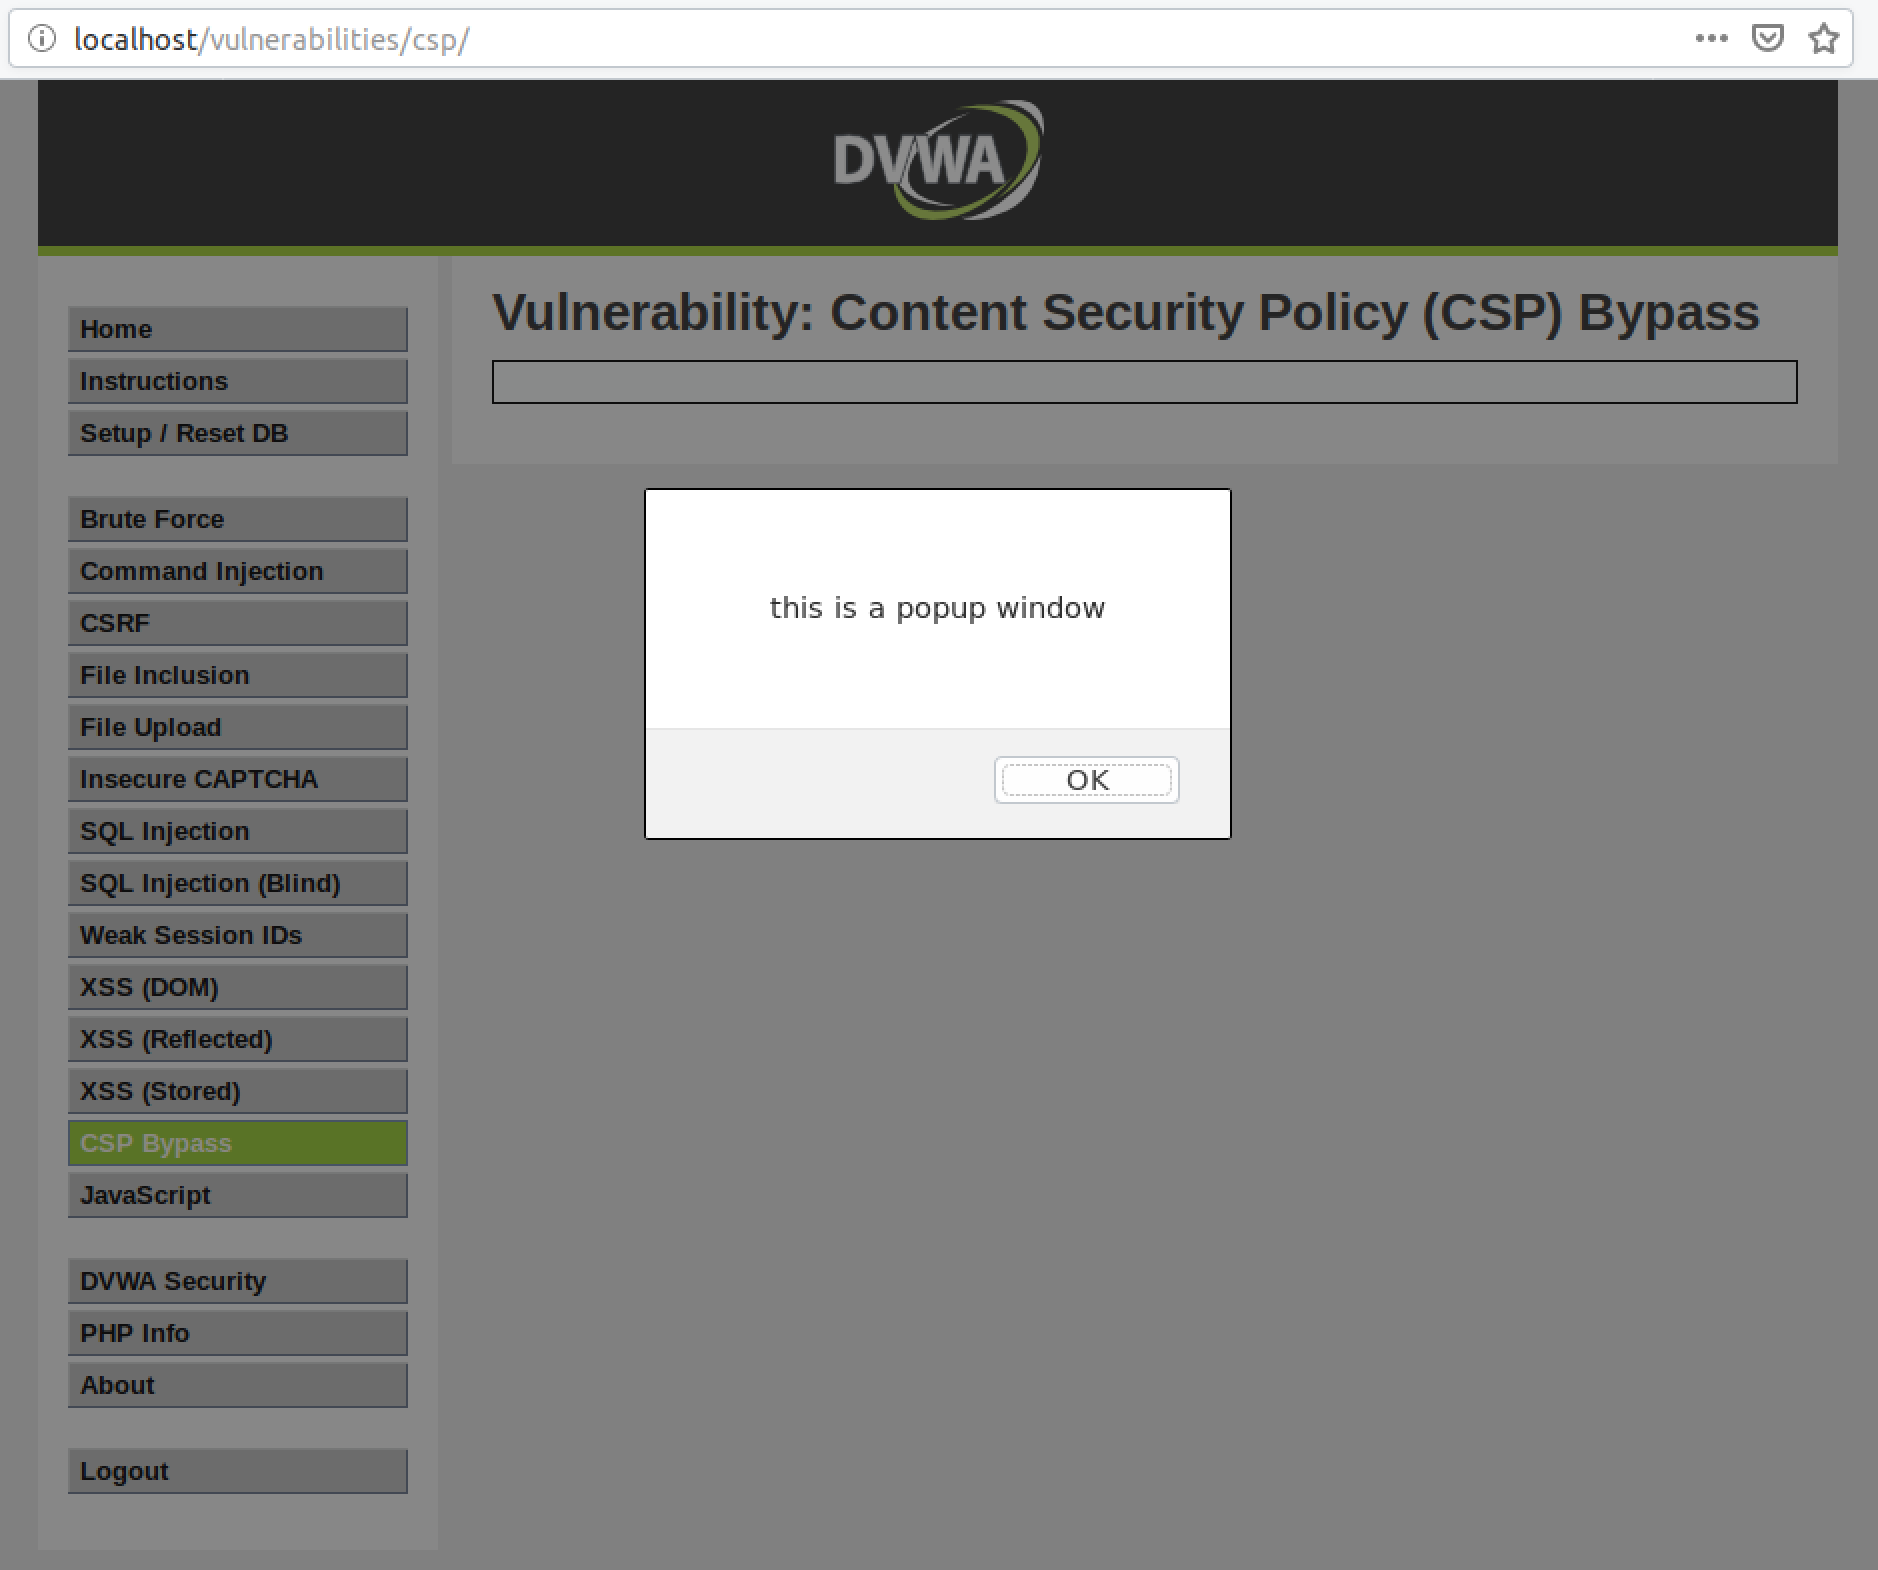
\includegraphics[width=.71\linewidth]{./csp_popup.png}
  \caption{\label{fig:CSP}
  Javascript popup from CSP vulnerability}
\end{figure}
\subsubsection*{SQL Injection}
On the SQL Injection tab, there were several steps needed to get the right information to access all the login credentials. First,
\begin{verbatim}
  %' OR '1'='1
\end{verbatim}
was entered to check if this would return all records that are false and all that are true, as well. The results are shown in
Figure~\ref{fig:SQL-1}, confirming that we can use the the previous input as a prefix to other inputs that query the rest of the
information. For example, the next input was
\begin{verbatim}
  %' AND 1=1 UNION SELECT null, table_name FROM
    INFORMATION_SCHEMA.tables #
\end{verbatim}
which returned information about all the other databases the server maintains, as shown in Figure~\ref{fig:SQL-2}. Next, changing the
input to
\begin{verbatim}
  %' and 1=1 UNION SELECT null, table_name FROM
    INFORMATION_SCHEMA.tables WHERE table_name LIKE 'user%' #
\end{verbatim}
returned and confirmed the table name needed to find login credentials, \verb|users|, shown in Figure~\ref{fig:SQL-3}. To get the
credentials, the input was changed to
\begin{verbatim}
  %' and 1=1 UNION SELECT null,
    concat(0x0a,user,0x0a,password) from users #
\end{verbatim}
The results of this are shown in Figure~\ref{fig:SQL-4} and include the username and hashed password at the bottom of each entry.
\begin{figure}[htbp]
  \centering
  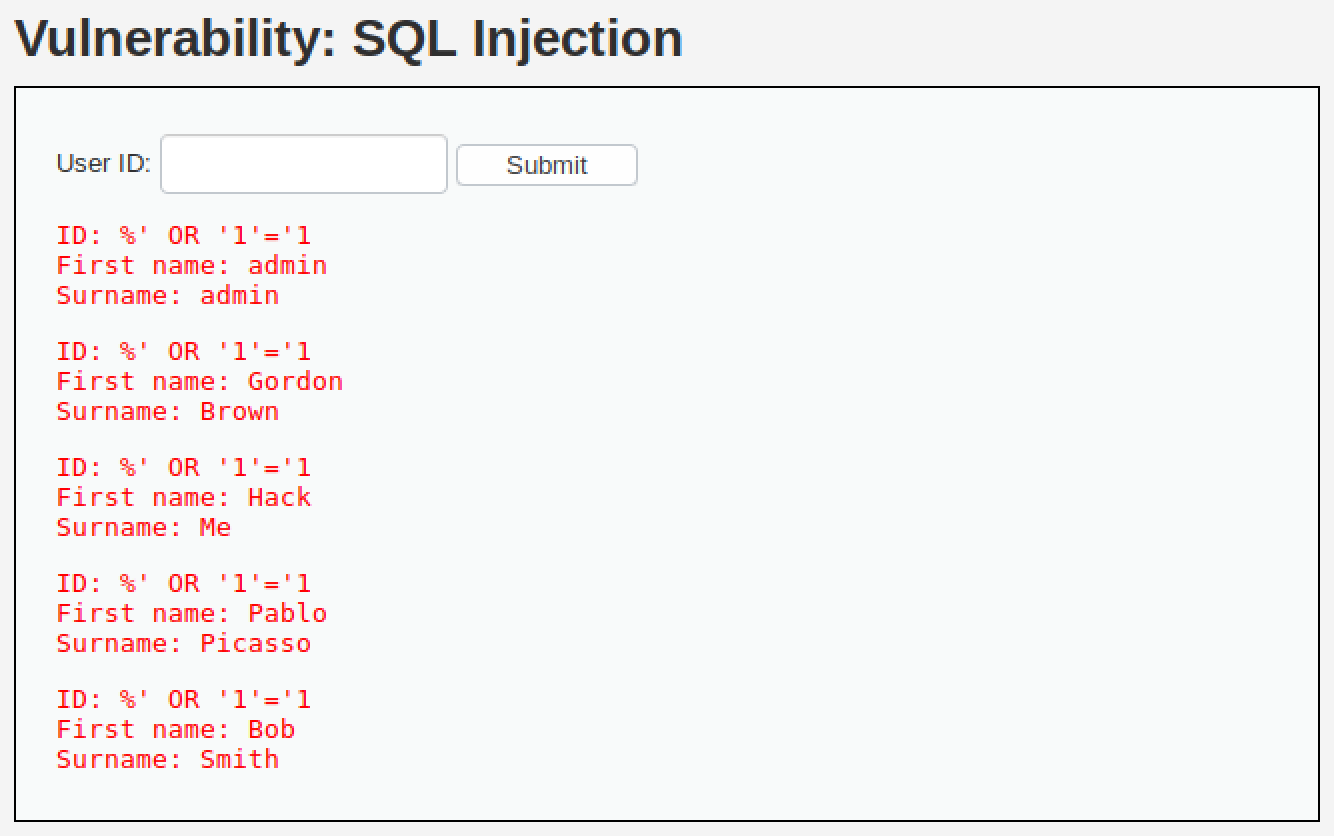
\includegraphics[width=1\linewidth]{./SQL-1.png}
  \caption{\label{fig:SQL-1}
  First SQL injection to check sanitization}
\end{figure}
\begin{figure}[htbp]
  \centering
  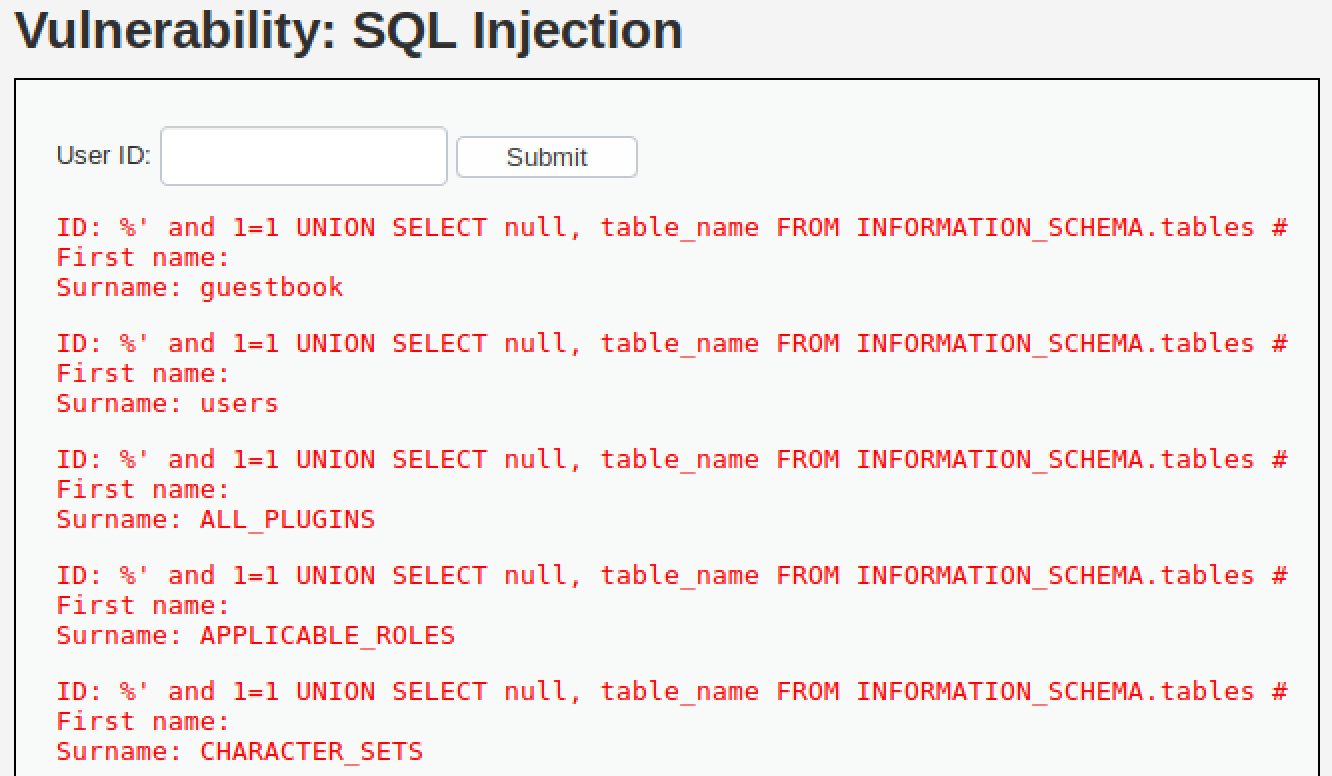
\includegraphics[width=1\linewidth]{./SQL-2.png}
  \caption{\label{fig:SQL-2}
  Result of query for table names (not all results shown)}
\end{figure}
\begin{figure}[htbp]
  \centering
  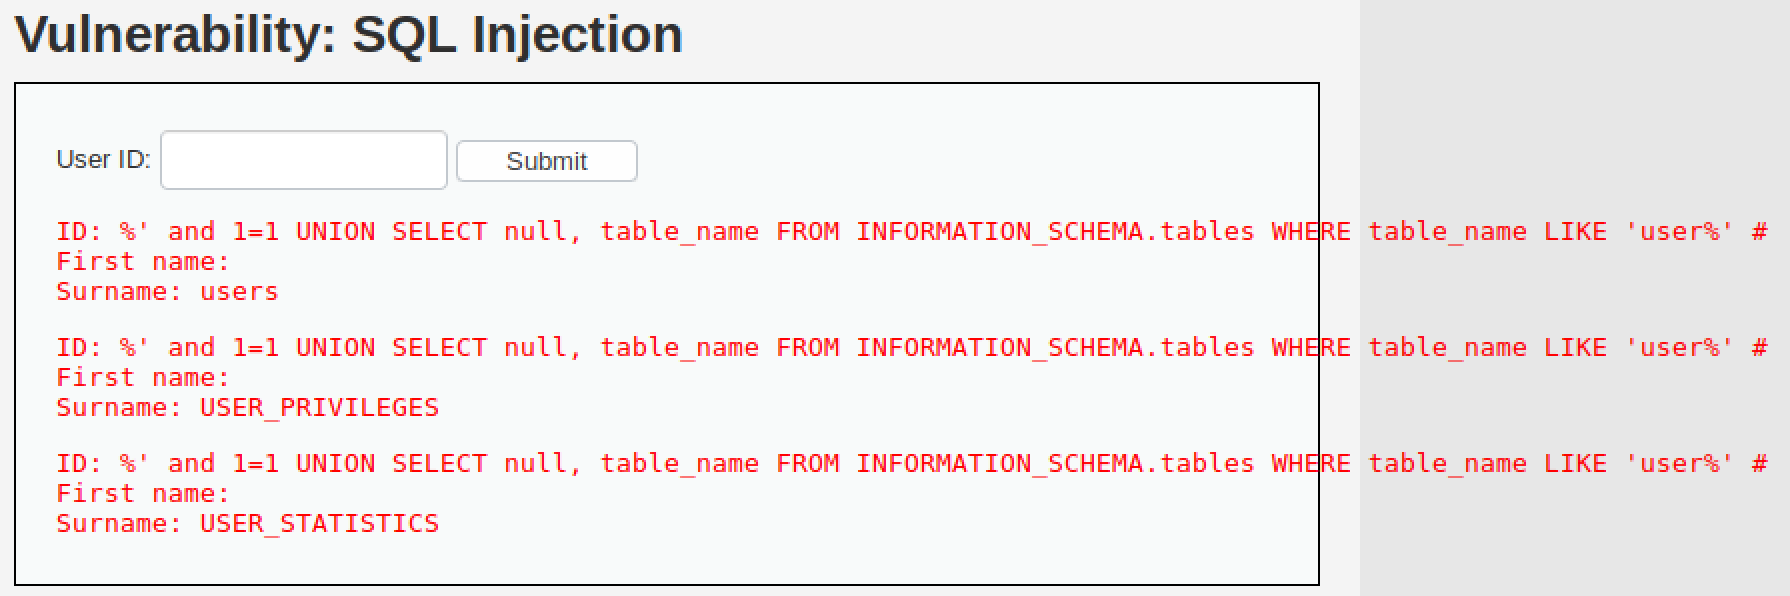
\includegraphics[width=1\linewidth]{./SQL-3.png}
  \caption{\label{fig:SQL-3}
  Result of query for table names similar to 'user'}
\end{figure}
\begin{figure}[htbp]
  \centering
  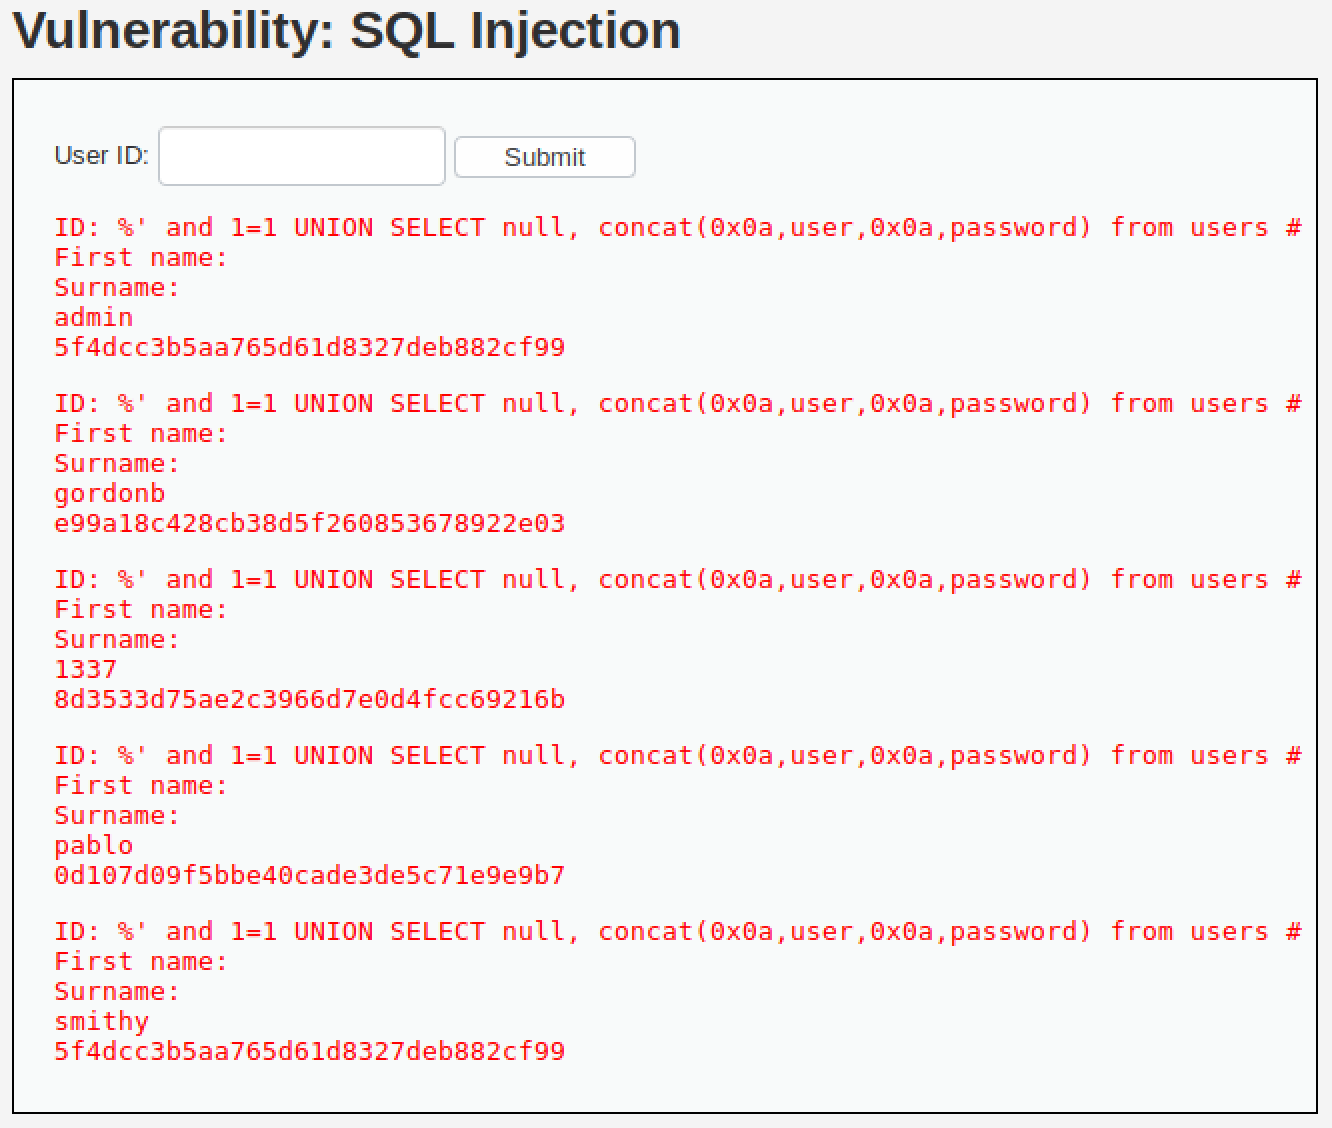
\includegraphics[width=1\linewidth]{./SQL-4.png}
  \caption{\label{fig:SQL-4}
  Result of query for user credentials}
\end{figure}\\
Using a website~\cite{md5} to decrypt the hashes, the login credentials of every user can be determined, as shown in Table~\ref{table:creds}.
\begin{table}[h]
  \centering
  \begin{tabular}{ |c|c|c|c|c|c| }
    \hline
    \textbf{USER:} & admin    & gordonb & 1337    & pablo   & smithy   \\ \hline
    \textbf{PASS:} & password & abc123  & charley & letmein & password \\ \hline
  \end{tabular}
  \caption{\label{table:creds}
  Table of credentials}
\end{table}
Since the input wasn't being sanitized, SQL queries could be submitted through the input box and then executed, returning all kinds
of information from the database. The queries at the beginning were to test what was valid and figure out the internal SQL query
that was being performed by the web app. Then, the table names could be queried using the \verb|INFORMATION_SCHEMA| table to find
the table name that was most likely to have user credentials. Once the right table is found, it becomes fairly simple to get the
hashed passwords and then decrypt it using a tool. The end result is the exposure of all these users' credentials.

Containerizing the web app limits what the attack can see and modify since the server is isolated from the actual host machine. This
is shown in the PHP injection where the results of \verb|ls /| and \verb=ps aux --no-headers | wc -l= are different when run from
the PHP script on the server and from the terminal of the VM hosting the container. However, containerizing doesn't prevent the
server itself from the kinds of attacks performed by bypassing the Content Security Policy and SQL injections. In other words,
the machine hosting the container is protected from attacks coming from inside the container, but the inside of the container is
still vulnerable.
\subsection*{1b - strace}
A method to detect exploits performed on DVWA is to use the tool \verb|strace|. It can attach to a process and log any system calls
that process makes. To monitor any system calls made by DVWA, \verb|strace| needs to be attached to a process called
\verb|containerd|. To get the PID of the process:
\begin{minted}{bash}
  $ ps -ef | grep containerd
  root     700    1  0 10:39 ?     00:00:00 /usr/bin/containerd
\end{minted}
Then, to attach \verb|strace| to the \verb|containerd| process and all of its children and run DVWA:
\begin{minted}{bash}
  $ sudo strace -p 700 -o strace.txt -f
  $ docker run --rm -it -p 80:80 vulnerables/web-dvwa
\end{minted}
Then, for example, the following command can be executed into the 'Command Injection' tab by closing off the \verb|ping| command with
a semicolon:
\begin{minted}{bash}
  ; echo "malware" > /tmp/maliciousfile
\end{minted}
The log produced from \verb|strace| in \verb|part1/strace.txt| can then be searched for system calls that create and write to 
that file:
\begin{minted}{bash}
  8545  execve("/bin/sh", ["sh", "-c", "ping  -c 4 ; echo
        \"malware\" > /t"... ], 0x7ffd96384018 /* 9 vars */
        <unfinished ... >
  ...
  8545  open("/tmp/maliciousfile",
        O_WRONLY|O_CREAT|O_TRUNC, 0666) = 3
  8545  fcntl(1, F_DUPFD, 10)             = 10
  8545  close(1)                          = 0
  8545  fcntl(10, F_SETFD, FD_CLOEXEC)    = 0
  8545  dup2(3, 1)                        = 1
  8545  close(3)                          = 0
  8545  write(1, "malware\n", 8)          = 8
  8545  dup2(10, 1)                       = 1
  8545  close(10)                         = 0
  8545  exit_group(0)                     = ?
  8545  +++ exited with 0 +++
\end{minted}
\subsection*{1c - Limiting network access with iptables}
First, \verb|firewalld| is masked and stopped to prevent it from being started by other services and tells the system to use
\verb|iptables|' rules. This is done using the following command:
\begin{minted}{bash}
  $ systemctl mask firewalld && systemctl stop firewalld
\end{minted}
Now the \verb|iptables| rules can be modified to only allow a single connection to the web server from \verb|10.157.90.8|.
This can be done with the following:
\begin{minted}{bash}
  $ sudo iptables \
      -A INPUT \          # append to chain INPUT
      -p tcp \            # specify protocol
      --dport 80 \        # specify port
      ! -s 10.157.90.8 \  # for all BUT specified source
      -j DROP             # DROP
\end{minted}
Now, any connections not from the specified IP are dropped. The new \verb|iptables| rules can be seen using:
\begin{minted}{bash}
  $ sudo iptables -S
\end{minted}
Alternatively, the output of \verb|iptables-save| can be saved into a file, which contains the rules as well, like in
\verb|part1/iptables.txt|.
\section*{Part 2 - SELinux}

\bibliography{bibliography}
\bibliographystyle{ieeetr}
\end{document}
